
% !TEX root = ./report.tex

% \subsection*{(a)}
% \subsubsection*{Method}

% 使用大小為 $d$ 的 dither matrix $I_d$,在圖片 $F$ 進行 dithering 的過程如下:
% \begin{enumerate}
%   \item 如果圖片長度 $N$ 不為 $d$ 的整數倍,則將圖片 padding 為 $N':=\left\lfloor\frac{N+d-1}{d}\right\rfloor*d$,即 $d$ 的倍數中不小於 $N$ 的最小者。對於寬度 $M$ 同理。
%   \item 計算 thresold matrix $T_d$,計算方式採用課堂投影片的 $$T_d(i,j):=255\cdot \frac{I_d(i,j)+0.5}{d^2}.$$
%   \item 將圖片分割為 $\frac{N'}{d}\cdot\frac{M'}{d}$ 個區塊。對於每個區塊,使用 $T_d$ 將區塊變為 binary image。即對於區塊 $F_{k,l}$,有
%         \[
%           G_{k,l}(i,j) = \begin{cases}
%             1, & F_{k,l}(i,j) \geq T_d(i,j) \\
%             0, & otherwise.
%           \end{cases}
%         \]

%   \item 最後將 $G_{k,l}$ 組合產生 $G$,最後輸出結果 $G[:N,:M]$,即去除 padding。
% \end{enumerate}

% 關於 $I_d$ 的計算方式留待下一小題討論。

% \subsubsection*{Result}
% \begin{figure}[!ht]
%   \centering
%   \begin{subfigure}[t]{.33\textwidth}
%     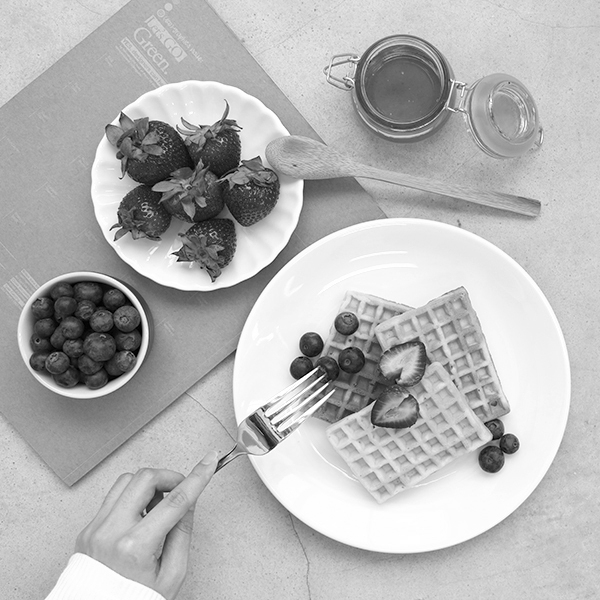
\includegraphics[width=0.9\linewidth]{../samples/sample1.png}
%     \caption{sample1}
%     \centering
%   \end{subfigure}
%   \begin{subfigure}[t]{.33\textwidth}
%     \centering
%     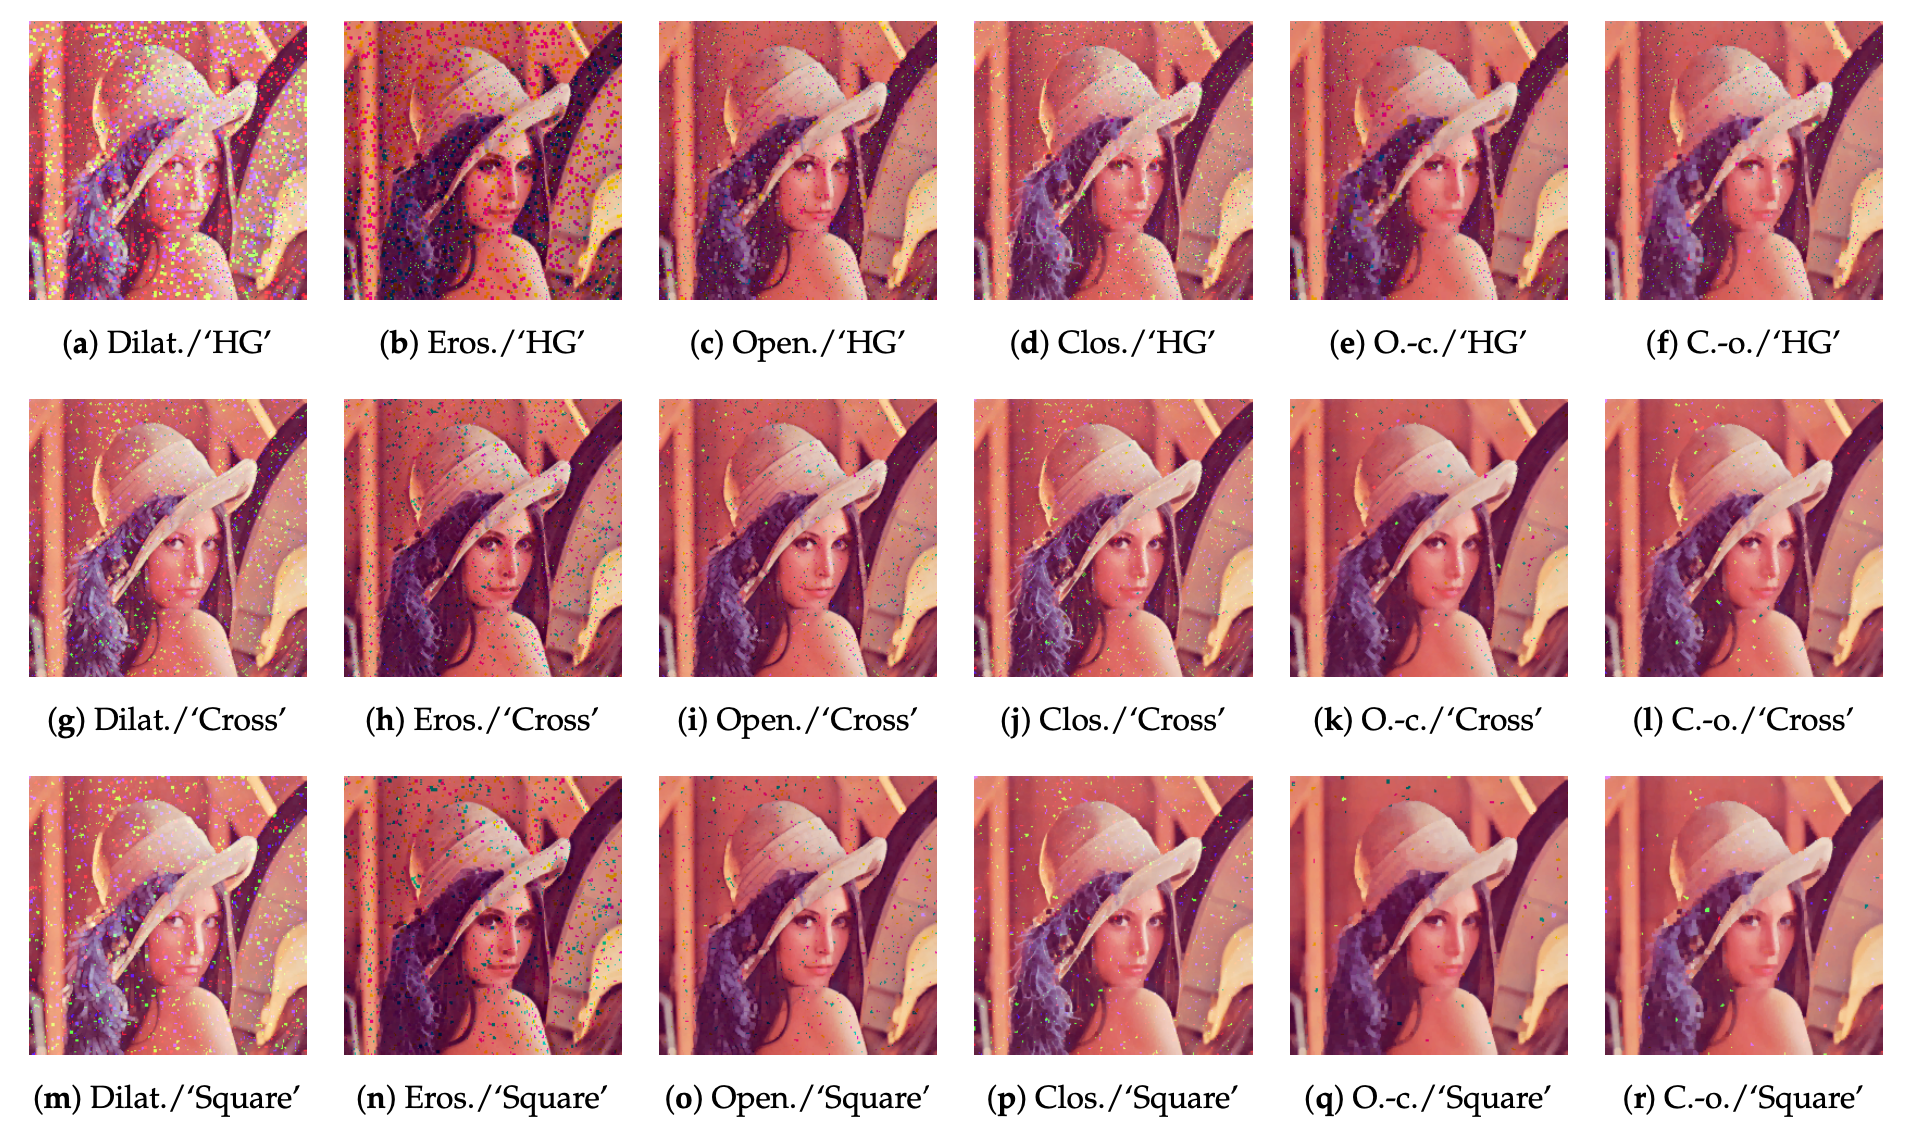
\includegraphics[width=0.9\linewidth]{../results/result1.png}
%     \caption{result1}
%   \end{subfigure}
% \end{figure}


% \subsection*{(b)}
% \subsubsection*{Method}

% 給定 $I_d$ 計算圖片 dithering 的方式已在上一小題提及,以下說明給定 $d=2^k$,其中 $k$ 為大於 $1$ 的正整數,如何計算 $I_d$。
% \begin{itemize}
%   \item 對於期望的輸出 $I_d$,將其分割為 4 等分計算。正式而言,令 $d'=\frac{d}{2}$,對於 $0\leq k,l \leq 1$,定義
%         \[
%           I_d^{k,l} := I_d[kd':(k+1)d',ld':(l+1)d'].
%         \]
%   \item 計算 $I_d^{k,l}$ 的公式為:
%         \[
%           I_d^{k,l}  = 4\cdot I_d'+I_2(k,l).
%         \]
%   \item 舉例而言,對於題目指定的 $I_2$,我們有
%         \[
%           I_{256} =\left[ \begin{array}{cc}
%               1\cdot I_{128}  & 2 \cdot I_{128} \\
%               3 \cdot I_{128} & 0\cdot I_{128}
%             \end{array} \right].
%         \]
% \end{itemize}

% \subsubsection*{Result}
% \begin{figure}[!ht]
%   \centering
%   \begin{subfigure}[t]{.33\textwidth}
%     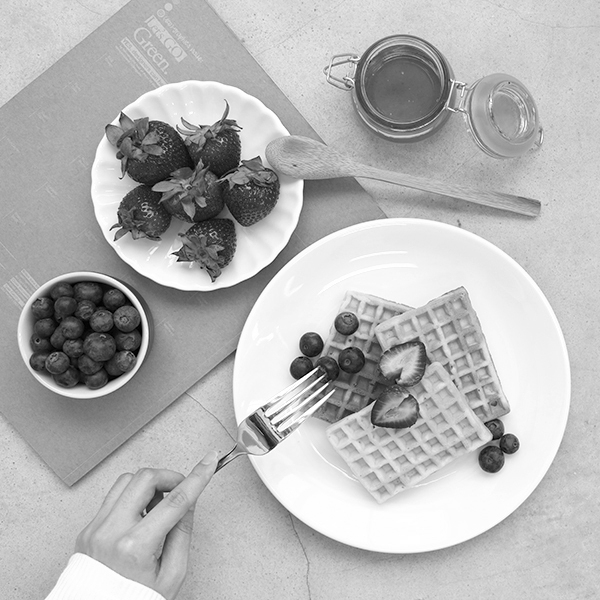
\includegraphics[width=0.9\linewidth]{../samples/sample1.png}
%     \caption{sample1}
%     \centering
%   \end{subfigure}
%   \begin{subfigure}[t]{.33\textwidth}
%     \centering
%     \includegraphics[width=0.9\linewidth]{../results/result2.png}
%     \caption{result2}
%   \end{subfigure}
% \end{figure}

% 另外,產生的 threshold matrix $T_{256}$ 如下:
% \begin{figure}[!ht]
%   \centering
%   \begin{subfigure}[t]{.33\textwidth}
%     \centering
%     \includegraphics[width=0.9\linewidth]{../refs/p1/a/dither256.png}
%     \caption{$T_256$}
%   \end{subfigure}
% \end{figure}

% \subsubsection*{Discussion}

% \clearpage
% \subsection*{(c)}
% \subsubsection*{Method}

% 為了方便起見,我對於 diffusion matrix 的定義和常見的有一點點不同,下文詳述。演算法如下所示:(迴圈有點多層,抱歉)

% \begin{algorithm}[!ht]
%   \caption{Error Diffusion}
%   \tcp{Index starts from 0.}

%   \Fn{\emph{\texttt{get\_center(img)}}}{
%     \Return{\emph{\texttt{(img.shape[0] // 2, img.shape[1] // 2)}}}
%   }

%   \Fn{\emph{\texttt{error\_diffusion(img, threshold, pattern)}}}{
%     \texttt{cur\_img $\defeq$ img.copy()}\;
%     \For{\emph{\texttt{i = 0 to img.shape[0]-1}}}{
%       \For{\emph{\texttt{j = 0 to img.shape[1]-1}}}{
%         \For{\emph{\texttt{k = 0 to pattern.shape[0]-1}}}{
%           \For{\emph{\texttt{l = 0 to pattern.shape[1]-1}}}{
%             \If{\emph{\texttt{cur\_img[i, j] < threshold}}}{
%               \texttt{error = cur\_img[i, j]}\;
%               \texttt{cur\_img[i, j] = 0}\;
%             }\Else{
%               \texttt{error = 255 - cur\_img[i, j]}\;
%               \texttt{cur\_img[i, j] = 255}\;
%             }

%             \;
%             \texttt{cx, cy} $\defeq$ \texttt{get\_center(pattern)}\;
%             \texttt{x, y} = \texttt{i-k-cx, j+l-cy}\;
%             \If{\emph{\texttt{img.is\_valid(x, y)}}}{
%               \texttt{cur\_img[x, y] += error * pattern[k, l]}\;
%             }
%           }
%         }
%       }
%     }

%     \Return{\emph{\texttt{cur\_img}}}\;
%   }
% \end{algorithm}

% 在上面的 pseudocode 中,我遍歷每個 \texttt{img} 中的像素,將 \texttt{pattern} 中心點對齊目前像素,並將 \texttt{pattern} 的值當作 weight 來將 \texttt{error} 擴散至周邊其他像素。

% 因此我所使用的 pattern matrix 分別如下:
% \begin{itemize}
%   \item Floyd-Steinberg:
%         \[
%           \left[ \begin{array}{ccc}
%               0 & 0 & 0 \\
%               0 & 0 & 7 \\
%               3 & 5 & 1
%             \end{array} \right]
%         \]
%   \item  Jarvis, Judice, Ninke:
%         \[
%           \left[ \begin{array}{cccccc}
%               0 & 0 & 0 & 0 & 0 \\
%               0 & 0 & 0 & 0 & 0 \\
%               0 & 0 & 0 & 7 & 5 \\
%               3 & 5 & 7 & 5 & 3 \\
%               1 & 3 & 5 & 3 & 1
%             \end{array} \right]
%         \]
% \end{itemize}


% \subsubsection*{Result}

% \begin{figure}[!ht]
%   \centering
%   \begin{subfigure}[t]{.3\textwidth}
%     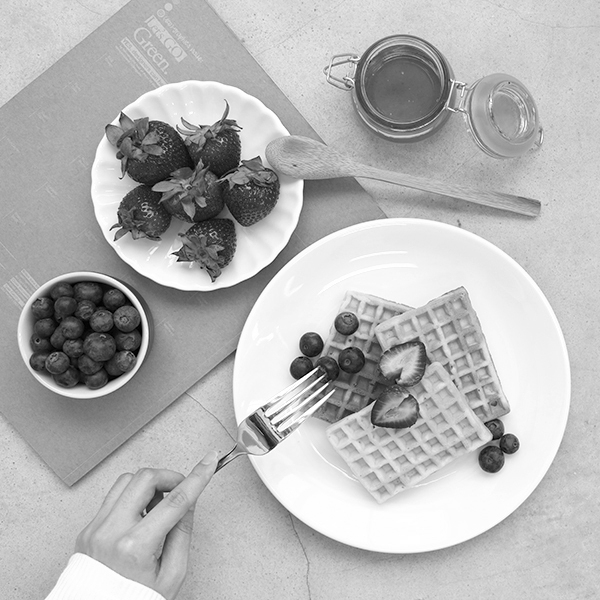
\includegraphics[width=0.9\linewidth]{../samples/sample1.png}
%     \caption{sample1}
%     \centering
%   \end{subfigure}
%   \begin{subfigure}[t]{.3\textwidth}
%     \centering
%     \includegraphics[width=0.9\linewidth]{../results/result3.png}
%     \caption{result3 (Floyd-Steinberg)}
%   \end{subfigure}
%   \begin{subfigure}[t]{.3\textwidth}
%     \centering
%     \includegraphics[width=0.9\linewidth]{../results/result4.png}
%     \caption{result4 (Jarvis)}
%   \end{subfigure}
% \end{figure}





